\documentclass[12pt]{article}
\usepackage{amssymb, amsmath, amsfonts, bm, graphicx, geometry}
\usepackage{tabularx, booktabs, float, enumitem, multicol, mathtools}
\usepackage{parskip} % Auto-manages paragraph spacing and removes indentations
\usepackage{siunitx, soul}  % Eases typesetting of numbers and units
\usepackage{mathrsfs}
\usepackage{amsthm}
\usepackage[most]{tcolorbox}

\geometry{margin=1in}
\newtcolorbox{definition}[1]{
    enhanced,
    breakable,
    colback=gray!5,
    colframe=black!60,
    boxrule=0.6pt,
    arc=2mm,
    left=1.5mm,
    right=1.5mm,
    top=1mm,
    bottom=1mm,
    fonttitle=\bfseries,
    title={Definition: #1}
}

\newtcolorbox{theorem}[1]{
    enhanced,
    breakable,
    colback=white,
    colframe=black,
    boxrule=0.8pt,
    borderline west={2pt}{0pt}{black},
    arc=1mm,
    left=2mm,
    right=1.5mm,
    top=1mm,
    bottom=1mm,
    fonttitle=\bfseries,
    title={Theorem: #1}
}

\begin{document}

\begin{center}
{\LARGE MA-224 Principles of Probability Notes\par}
\end{center}
\hrule
\vspace{1.5em}
Probability is not statistics! Probability is the study of random events and how likely they are to occur, while statistics studies the data that results from those events. In other words, probability predicts while statistics analyzes past information.
\section*{\fbox{Introduction to and properties of
probability (1.1-1.2)}}
\subsection*{\underline{1.1 Basic Concepts}}
\begin{definition}{Random Experiment}
A random experiment is an experiment whose outcome cannot be predicted with certainty \textit{before it is performed}.\\\\
\underline{Ex:} Flipping a coin is a random experiment. The possible outcomes are heads or tails, but you cannot predict which one will occur before the coin is flipped.
\end{definition}

\begin{definition}{Outcome}
An outcome is one possible result of a random experiment.\\\\
\underline{Ex:} In a 6-sided die roll, the possible outcomes are 1, 2, 3, 4, 5, or 6.
\end{definition}

\begin{definition}{Sample Space}
The sample space, also called the \textbf{outcome space} or \textbf{space} $S$, is the set of all possible outcomes of a random experiment.
\[S = \{ \text{all possible outcomes} \}\]
The sample space can be finite, countably infinite, or continuous.\\\\
\underline{Ex 1:} Coin flip: $S = \{H, T\}$\\
\underline{Ex 2:} 6-sided die roll: $S = \{1, 2, 3, 4, 5, 6\}$\\
\underline{Ex 3:} Roll two 6-sided dice and sum the results: $S = \{2, 3, 4, 5, 6, 7, 8, 9, 10, 11, 12\}$\\
\end{definition}

\begin{definition}{Random Variable}
A random variable assigns a numerical value to each outcome of a random experiment. It converts outcomes into numbers that could be analyzed.\\\\
A more rigorous definition is that, given a random experiment with sample space $S$, a random variable $X$ is a function
\[
X:S\to\mathbb{R},
\]
which assigns a real number $X(s)$ to each outcome $s\in S$.\\\\
Note that $X:S\to\mathbb{R}$ means that $X$ is a function that takes an input from the sample space $S$ and outputs a real number in $\mathbb{R}$.\\\\
\underline{Ex 1:} Flip a coin twice: $S = \{HH, HT, TH, TT\}$\\
Define a random variable $X$ that counts the number of heads in the outcome. Then:
\[X(HH) =2, \quad X(HT) =1, \quad X(TH) =1, \quad X(TT) =0\]
A random variable can be discrete or continuous.
\begin{itemize}
    \item \textbf{Discrete random variable:} A random variable is discrete when its possible values can be listed as a finite or countably infinite set.
    \item \textbf{Continuous random variable:} A random variable is continuous when its possible values range over an interval rather than being individually countable.
\end{itemize}
\vspace{1em}
\underline{Ex 2:} The random variable $X\in{0,1,2}$ in Ex 1 is discrete. However, if we consider the random variable $Y$ that measures weight in pounds of a randomly selected person, then $Y$ is continuous.
\end{definition}


\begin{definition}{Frequency}
    If we repeat a random experiment $n$ times, and a certain outcome $A$, occurs $f=\mathcal{N}(A)$ times, then the number $f$ is called the \textbf{frequency} of the outcome $A$. \\\\
    \underline{Ex 1:} If we roll a 6-sided die 7 times and get the outcome 4 three times, then the frequency of the outcome 4 is $f=3$.
\end{definition}

\begin{definition}{Relative Frequency}
    The relative frequency of an outcome $A$ is the ratio of the frequency of $A$ to the total number of trials $n$. In other words, it is the normalized frequency of the outcome $A$.
    \[\text{(Relative Frequency)} = \frac{f}{n} = \frac{\mathcal{N(A)}}{n}\]
    \underline{Ex 1:} If we roll a 6-sided die 20 times and get the outcome 4 five times, then the relative frequency of rolling a 4 is:
    \[\frac{N(4)}{n}=\frac{5}{20}\]
\end{definition}
A visual way to present relative frequency is through a histogram. For example, see the following relative frequency histogram $h(x)$ and frequency table for the number of children in 100 families:
\begin{center}
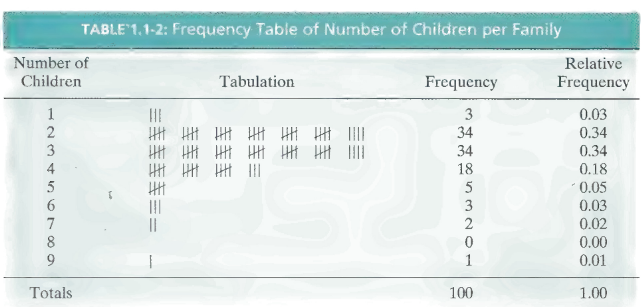
\includegraphics[width=0.7\textwidth]{1.1 histogram.png}
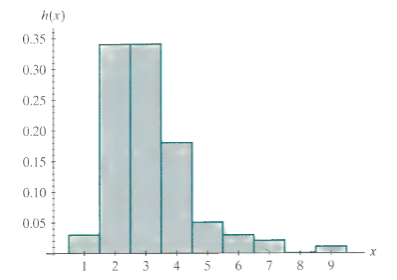
\includegraphics[width=0.5\textwidth]{1.1 histogram 2.png}
\end{center}
Note that for a regular histogram:
\begin{itemize}
    \item x-axis: the possible values of the random variable
    \item y-axis: the frequency of each value
\end{itemize}
For a relative frequency histogram:
\begin{itemize}
    \item x-axis: the possible values of the random variable
    \item y-axis: the relative frequency of each value
\end{itemize}

\begin{definition}{Probability Mass Function (p.m.f.)}
    For a discrete random variable $X$, the probability mass function (p.m.f.) is a function that assigns a probability to every possible value of $X$.
    \[f(x) = P(X = x)\]
    \hl{A p.m.f. is different from a probability. A probability is a numerical value assigned to an event, while a p.m.f. is a function that gives the probability associated with each possible value of a discrete random variable.} Note that random variable definitions matter a lot in the context of p.m.f.\\\\
    \underline{Ex 1:} For a fair 6-sided die roll, the p.m.f. is:
    \[
f(x)=
\begin{cases}
\dfrac{1}{6}, & x\in\{1,2,3,4,5,6\},\\[4pt]
0, & \text{otherwise}.
\end{cases}
\]
    Since the die is fair, each outcome has an equal probability of $\frac{1}{6}$.\\\\

    \underline{Ex 2:} Flip two fair coins and let $X$ be the number of heads obtained.

\[
f(x)=
\begin{cases}
\dfrac{1}{4}, & x=0,\\[4pt]
\dfrac{1}{2}, & x=1,\\[4pt]
\dfrac{1}{4}, & x=2,\\[4pt]
0, & \text{otherwise}.
\end{cases}
\]

This is because the sample space is
\[
S=\{HH,HT,TH,TT\},
\]
so
\[
P(X=0)=\frac14,\qquad
P(X=1)=\frac24=\frac12,\qquad
P(X=2)=\frac14.
\]
\end{definition}
Now using the p.m.f., we can also graphically represent the probabilities of each outcome using a probability histogram $f(x)$. Where:
\begin{itemize}
    \item x-axis: the possible values of the random variable
    \item y-axis: the probability of each value
\end{itemize}
See the following comparison of the probability histogram $f(x)$ and the relative frequency histogram $h(x)$ for a random experiment:
\begin{center}
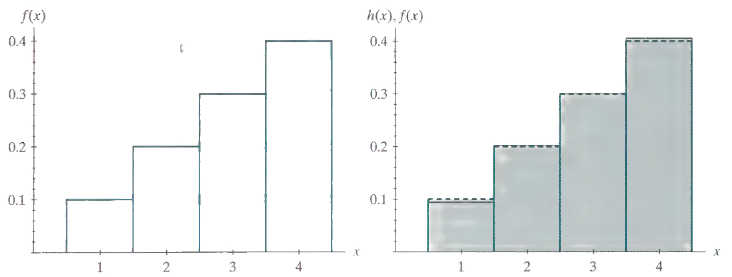
\includegraphics[width=0.7\textwidth]{1.1 prob histogram.png}
\end{center}
As the number of trials $n$ increases, the relative frequency histogram $h(x)$ approaches the probability histogram $f(x)$. 
\begin{definition}{Mode}
    The mode is the value of \(x\) having the greatest probability, or equivalently the highest relative frequency in observed data.\\\\
    \underline{Ex 1:} Suppose a random variable \(X\) has the following p.m.f.:
    \[f(1) = 0.1, \quad f(2) = 0.3, \quad f(3) = 0.4, \quad f(4) = 0.2\]
    The mode of \(X\) is \(3\), since it has the highest probability of \(0.4\).
\end{definition}

\subsection*{\underline{1.2 Properties of Probability}}
\begin{definition}{Event}
An event is a \hl{subset of the sample space}. It is a collection of one or more outcomes of a random experiment that satisfies a certain condition.\\\\
When the random experiment is performed and the outcome of the experiment is in $A$, we say that the event $A$ has occurred.\\\\
\underline{Ex 1:} For a 6-sided die roll: $S = \{1, 2, 3, 4, 5, 6\}$\\
The event of rolling an even number is $A = {\text{roll is even}} = \{2, 4, 6\}$\\\\
\underline{Ex 2:} Flip a coin twice: $S = \{HH, HT, TH, TT\}$\\
The event of getting at least one head is $B = {\text{at least one head}} = \{HH, HT, TH\}$\\
\end{definition}
\subsection*{Algebra of Sets}
\begin{itemize}
    \item $\varnothing$ denotes the \textbf{null} or \textbf{empty set};
    \item $A \subset B$ means $A$ is a \textbf{subset} of $B$;
    \begin{itemize}
        \item ALL outcomes in $A$ are also in $B$
    \end{itemize}
    \item $A \cup B$ is the \textbf{union} of $A$ and $B$:
    \begin{itemize}
        \item All the outcomes in $A$ or $B$ or both; If the problem states \hl{"$A$ or $B$"}, it is referring to the union of $A$ and $B$.
    \end{itemize}
    \item $A \cap B$ is the \textbf{intersection} of $A$ and $B$;
    \begin{itemize}
        \item Only outcomes that are in both $A$ and $B$; If the problem states \hl{"$A$ and $B$"}, it is referring to the intersection of $A$ and $B$.
    \end{itemize}
    \item $A \setminus B$ is the \textbf{set difference} of $A$ and $B$;
    \begin{itemize}
        \item All outcomes in $A$ that are NOT in $B$. For example, if $A = \{1, 2, 3\}$ and $B = \{2, 3, 4\}$, then $A \setminus B = \{1\}$.
        \item Note that the following is equivalent: $A \setminus B = A \cap B'$, where $B'$ is the complement of $B$. (Since $B'$ contains all outcomes that are not in $B$ by definition, the intersection of $A$ and $B'$ will contain all outcomes that are in $A$ but not in $B$.)
    \end{itemize}
    \item $A'$ is the \textbf{complement} of $A$ (i.e., all elements in $S$ that are not in $A$).
    \begin{itemize}
        \item Some other notation for the complement of $A$ is $A^c$ or $\overline{A}$. $A'$ can also be thought of as the set difference between the sample space and the event\\\\
        i.e., $A' = S \setminus A$ (contains all possible outcomes that are not in $A$). For example, if $S = \{1, 2, 3, 4, 5\}$ and $A = \{2, 3\}$, then $A' = \{1, 4, 5\}$.
    \end{itemize}
\end{itemize}
Some of the sets above can be visualized using a Venn diagram:
\begin{center}
    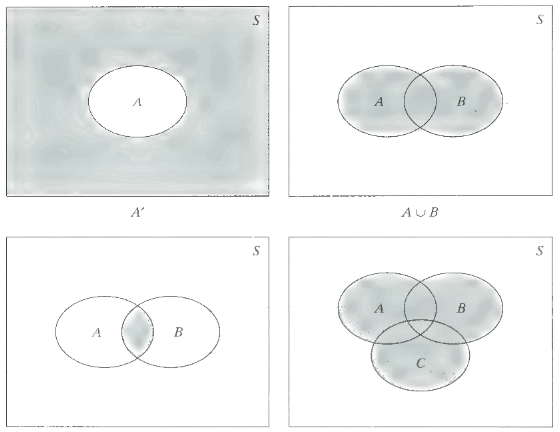
\includegraphics[width=0.7\textwidth]{1.2 venn diagram.png}
\end{center}
\begin{itemize}
    \item \textbf{Commutative laws} (order doesn't matter):
    \[
    A \cup B = B \cup A
    \]
    \[
    A \cap B = B \cap A
    \]

    Example: if
    \[
    A=\{1,2\}, \qquad B=\{2,3\},
    \]
    then
    \[
    A\cup B=\{1,2,3\}=B\cup A
    \]
    and
    \[
    A\cap B=\{2\}=B\cap A.
    \]

    \item \textbf{Associative laws} (grouping doesn't matter):
    \[
    (A\cup B)\cup C=A\cup(B\cup C)
    \]
    \[
    (A\cap B)\cap C=A\cap(B\cap C)
    \]

    Example: if
    \[
    A=\{1,2\},\quad B=\{2,3\},\quad C=\{2,4\},
    \]
    then
    \[
    (A\cup B)\cup C
    =\{1,2,3,4\}
    =A\cup(B\cup C),
    \]
    and
    \[
    (A\cap B)\cap C
    =\{2\}
    =A\cap(B\cap C).
    \]

    \item \textbf{Distributive laws} (distribute one operation through another):
    \[
    A\cap(B\cup C)
    =(A\cap B)\cup(A\cap C)
    \]
    \[
    A\cup(B\cap C)
    =(A\cup B)\cap(A\cup C)
    \]

    Example: let
    \[
    A=\{1,2\},\quad B=\{2,3\},\quad C=\{1,3\}.
    \]
    Then
    \[
    A\cap(B\cup C)
    =\{1,2\},
    \]
    while
    \[
    (A\cap B)\cup(A\cap C)
    =\{2\}\cup\{1\}
    =\{1,2\}.
    \]

    \item \textbf{Identity laws} (ways to combine a set such that it remains unchanged):
    \[
    A\cup\varnothing=A
    \]
    \[
    A\cap S=A
    \]

    \item \textbf{Domination laws} (one set "takes over" the result):
    \[
    A\cup S=S
    \]
    \[
    A\cap\varnothing=\varnothing
    \]

    \item \textbf{Idempotent laws} (combining a set with itself doesn't change it):
    \[
    A\cup A=A
    \]
    \[
    A\cap A=A
    \]

    \item \textbf{Complement laws} (a set combined with everything outside it):
    \[
    A\cup A'=S
    \]
    \[
    A\cap A'=\varnothing
    \]
\end{itemize}

\begin{theorem}{DeMorgan's Laws}
    For a finite number of sets $A_1, A_2, \ldots, A_n$ in a sample space $S$, the following hold:
    \begin{enumerate}
        \item $$\left(\bigcup_{i=1}^{n} A_i\right)' = \bigcap_{i=1}^{n} A_i'$$
        \item $$\left(\bigcap_{i=1}^{n} A_i\right)' = \bigcup_{i=1}^{n} A_i'$$
    \end{enumerate}
    For example, for two sets $A$ and $B$, we have:
     \[
    (A\cup B)'=A'\cap B'
    \]
    \[
    (A\cap B)'=A'\cup B'
    \]
    In other words, the complement flips the union and intersections of a finite number of sets.
    \begin{center}
    \includegraphics[width=0.7\textwidth]{1.2 demorgans.png}
    \end{center}
\end{theorem}

\begin{definition}{Mutually Exclusive Events}
    We say $A_1, A_2, \ldots, A_n$ in a sample space $S$ are \textbf{mutually exclusive} if no two events can occur at the same time. In other words, the intersection of any two events is empty:
    \[
    A_i \cap A_j = \varnothing \quad \text{for all } i \neq j.
    \]
    In other words, events $A$ and $B$ are mutually exclusive if they cannot occur at the same time.\\\\
    \underline{Ex 1:} For a 6-sided die roll, let $A = \{\text{roll is even}\} = \{2, 4, 6\}$ and $B = \{\text{roll is odd}\} = \{1, 3, 5\}$. Then $A$ and $B$ are mutually exclusive since
    \[
    A \cap B = \varnothing.
    \]
    Note that mutually exclusive events are also called \textbf{disjoint} events.
\end{definition}

\begin{definition}{Exhaustive Events}
    We say $A_1, A_2, \ldots, A_n$ in a sample space $S$ are \textbf{exhaustive} if their union covers the entire sample space:
    \[
    \bigcup_{i=1}^{n} A_i =A_1 \cup A_2 \cup \cdots \cup A_n = S.
    \]
    In other words, \textit{at least} one of the events must occur.
\\\\
\underline{Ex 1:} For a 6-sided die roll, let $A = \{\text{roll is even}\} = \{2, 4, 6\}$ and $B = \{\text{roll is odd}\} = \{1, 3, 5\}$. Then $A$ and $B$ are mutually exhaustive since
    \[
    A \cup B = S.
    \]
\end{definition}

\begin{definition}{Partition of a Sample Space}
    If $A_1, A_2, \ldots, A_n$ are \hl{mutually exclusive and exhaustive events} in a sample space $S$, then we say that $\{A_1, A_2, \ldots, A_n\}$ is a \textbf{partition} of the sample space $S$.\\\\
    In other words, the sets don't overlap (mutually exclusive) and together they cover the entire sample space (exhaustive).\\\\
    \underline{Ex 1:} Let
\[
S=\{1,2,3,4,5,6\}.
\]
A partition of \(S\) is
\[
\big\{\{1,2\},\{3,4\},\{5,6\}\big\}
\]
The subsets are mutually exclusive because they don't overlap:
\[
\{1,2\}\cap\{3,4\}=\varnothing,
\]
and similarly for the other pairs.\\\\
Their union is the entire set:
\[
\{1,2\}\cup\{3,4\}\cup\{5,6\}=S.
\]
\end{definition}

\begin{definition}{Probability Measure}
    A probability measure is a function $P$ that assigns a real number $P(A)$ to each event $A$ in a sample space $S$ ($P:S\to\mathbb{R}$) such that it satisfies the following axioms:
    \begin{enumerate}
        \item $0 \leq P(A)$ for any event $A$ in $S$. (The probability of any event is non-negative)
        \item $P(S) = 1$. (\textit{Something} has to happen)\\\\
        This naturally places the upper bound of the probability of any event at 1, since $A\subset S$ implies $P(A)\leq P(S)=1$.
        \item For a finite set of events $A_1, A_2, \ldots, A_n$, we can sum their probabilities the following way \hl{if and only if they are mutually exclusive (no overlaps: no double counting!)}:
        \[
        P(A_1 \cup A_2 \cup \cdots \cup A_n) = P(A_1) + P(A_2) + \cdots + P(A_n).
        \]
        \[\implies P \left(\bigcup_{i=1}^{n} A_i\right) = \sum_{i=1}^{n} P(A_i)\]
    \end{enumerate}
\end{definition}

\begin{theorem}{Properties of Probability}
\textbf{Property 1}\\
For any event $A$ in a sample space $S$ ($A\subset S$):
\[P(A) = 1 - P(A')\]
\textit{Proof:} Since $A$ and $A'$ are mutually exclusive, $A \cap A' = \varnothing$, and they are exhaustive, $A \cup A' = S$. By axiom 3 of probability measure we can sum their probabilities:
\[P(A \cup A') = P(A) + P(A')\]
Since $A \cup A' = S$, we have:
\[P(S) = P(A) + P(A')\]
Since $P(S) = 1$ by axiom 2 of probability measure,
\[1 = P(A) + P(A')\]
Therefore:
\[P(A) = 1 - P(A')\]
\textbf{Property 2}\\
The probability of the empty set is zero (something must happen):
\[P(\varnothing) = 0\]
\textit{Proof:} Since $\varnothing' = S$, we can use property 1 and axiom 2 of probability measure to show that:
\[P(\varnothing) = 1 - P(\varnothing') = 1 - P(S) = 1 - 1 = 0\]
\textbf{Property 3}\\
If $A\subset B$, then
\[P(A) \leq P(B)\]
\textit{Proof:} We can rewrite $B$ as the union of $A$ and the set difference $B \setminus A$:
\[B = A \cup (B \setminus A)\]
(Outcomes in $A$ + outcomes in $B$ that are not in $A$ = all outcomes in $B$)\\\\
Since $A$ and $B \setminus A$ are mutually exclusive ($A \cap (B \setminus A ) = \varnothing$), we can use axiom 3 of probability measure to sum their probabilities:
\[P(B) = P(A) + P(B \setminus A)\]
Since $P(B \setminus A) \geq 0$ by axiom 1 of probability measure, we have:
\[P(B) \geq P(A)\]
\textbf{Property 4}\\
For any event $A$ in a sample space $S$:
\[P(A) \leq 1\]
\textit{Proof:} We lowkey already proved this since $A\subset S$ implies $P(A)\leq P(S)=1$ by property 3 of probability.\\\\
\textbf{Property 5 \hl{(Principle of Inclusion-Exclusion: PIE)}}\\
Let $A$ and $B$ be any two events in a sample space $S$ (not necessarily mutually exclusive, could overlap $\leftarrow$ omg double counting?). Then the probability of the union of $A$ and $B$ is given by:
\[P(A \cup B) = P(A) + P(B) - P(A \cap B)\]
\textit{Proof:} We can rewrite $A \cup B$ as the union of $A$ and the set difference $B \setminus A$:
\[A \cup B = A \cup (B \setminus A)\]
and rewrite since $A$ and $B \setminus A$ are mutually exclusive,
\[A\cap(B\setminus A) = \varnothing\]
By axiom 3 of probability measure, we can sum their probabilities:
\[P(A \cup B) = P(A) + P(B \setminus A) \quad \text{(eqn 1)}\]
\hl{Here's the trick!} We can also rewrite $B$ as the union of $B \setminus A$ and the intersection $A \cap B$:
\[B = (B \setminus A) \cup (A \cap B)\]
Since $B \setminus A$ and $A \cap B$ are mutually exclusive,
\[(B \setminus A) \cap (A \cap B) = \varnothing\]
Putting it all together, we can sum their probabilities by axiom 3 of probability measure:
\[P(B) = P(B \setminus A) + P(A \cap B)\]
Rearranging, we have:
\[P(B \setminus A) = P(B) - P(A \cap B)\]
Substituting this into equation (1), we have:
\[P(A \cup B) = P(A) + P(B \setminus A) = P(A) + P(B) - P(A \cap B)\]
Essentially, when we sum two overlapping events, we \textit{double count} their intersection (since both $A$ and $B$ contain the outcomes in $A \cap B$), so we need to subtract it out to get the correct probability of the union.
\end{theorem}
\begin{theorem}{PIE for 3}
    Let $A$, $B$, and $C$ be any three events in a sample space $S$. Then the probability of the union of $A$, $B$, and $C$ is given by:
    \[
\begin{aligned}
P(A \cup B \cup C)
&= P(A) + P(B) + P(C) \\
&\quad - P(A \cap B) - P(A \cap C) - P(B \cap C) \\
&\quad + P(A \cap B \cap C)
\end{aligned}
\]
Similar to PIE for 2 events, we need to first subtract the pairwise intersections to correct for double counting (there are three sets, so three pairwise intersections), but then we are missing the triple intersection, which we need to add back in to correct for triple counting.
\begin{center}
    \includegraphics[width=0.6\textwidth]{1.2 PIE for 3.png}
\end{center}
\end{theorem}
\subsection*{\fbox{Counting! (1.3)}}
\subsection*{\underline{1.3 Methods of Enumeration}}
The main focus of this section is to learn how to count the number of possible outcomes for a random experiment. This is VERY important because the probability of an event is defined as the ratio of the number of favorable outcomes to the total number of possible outcomes! But first some definitions:
\begin{definition}{Ordered sample}
    An ordered sample is a selection in which the order of the selected objects matters. In other words, different arrangements of the same objects are considered different outcomes.\\\\
    \underline{Ex 1:} Consider the set $\{A, B, C\}$. The following ordered samples of size 3 are considered different outcomes:
    \[ABC, ACB, BAC, BCA, CAB, CBA\]
\end{definition}

\begin{definition}{Distinct Objects}
   Distinct objects are objects that are treated as different from one another and are distinguishable. \hl{People are always distinct!}\\\\
    In other words, if two objects are distinct, we get a different outcome/ordering if we swap them. If two objects are not distinct, we get the same outcome/ordering if we swap them.\\\\
    \underline{Ex 1:} Consider the set $\{A, B, C\}$. If $A$, $B$, and $C$ are distinct objects, then $ABC$ and $BAC$ are considered different outcomes. However, if $A$ and $B$ are not distinct (i.e., they are the same object), then $ABC$ and $BAC$ are considered the same outcome.
\end{definition}

\begin{definition}{Sampling With Replacement}
    In sampling with replacement, an object is returned before the next selection, so it can be selected again.\\\\
    \hl{The total number of objects stays the same between successive selections!}
\end{definition}

\begin{definition}{Sampling Without Replacement}
    In sampling without replacement, an object is not returned before the next selection, so it cannot be selected again.\\\\
    \hl{The total number of objects decreases between successive selections!}
\end{definition}
Usually a counting problem can be broken down into a series of simpler counting problems. Two ways this can be down is through the addition principle and the multiplication principle.
\begin{theorem}{Addition Principle}
Suppose we have $\ell$ mutually exclusive events $A_1, A_2, \ldots, A_\ell$. Then the total number of outcomes in the union of these events is given by:
\[|A_1 \cup A_2 \cup \cdots \cup A_\ell| = |A_1| + |A_2| + \cdots + |A_\ell|\]
Where the notation $|A|$ denotes the \hl{number of outcomes in the event $A$}.\\\\
In other words, if we can split a single counting problem into a finite number of mutually exclusive cases, we can count the number of outcomes in each case and sum them to get the total number of outcomes.\\\\
We call the events $A_1, A_2, \ldots, A_\ell$ \textbf{cases}. They shouldn't overlap (mutually exclusive) and ideally should be easy to count!\\\\
\underline{Ex 1:} Bowl of 3 toys: 1 red, 1 blue, 1 purple. How many different ways can we select toys?\\\\
We can split this counting problem into 4 mutually exclusive cases:
\begin{itemize}
    \item Case 0: No toys selected: 1 way
    \item Case 1: 1 toy selected: 3 ways (red, blue, purple)
    \item Case 2: 2 toys selected: 3 ways (red+blue, red+purple, blue+purple)
    \item Case 3: 3 toys selected: 1 way (red+blue+purple)
\end{itemize}
By the addition principle, the total number of subsets is:
\[|A_0 \cup A_1 \cup A_2 \cup A_3| = |A_0| + |A_1| + |A_2| + |A_3| = 1 + 3 + 3 + 1 = 8\] 
\end{theorem}

\begin{theorem}{Multiplication Principle}
    A counting problem can also be broken into successive \textbf{stages}. \hl{Each stage represents a potential decision we make in the selection.} Consider if each stage $i$ has $r_i$ outcomes ($r_i$ has to be independent of the outcomes of the previous stages). Then the total number of outcomes in the counting problem is given by:
    \[r_1 \cdot r_2 \cdot r_3 \cdots r_n\]
    \underline{Ex 1:} Bowl of 3 toys: 1 red, 1 blue, 1 purple. How many different ways can we select toys?
    \begin{itemize}
        \item Stage 1: Did I select the red toy? 2 outcomes (yes or no)
        \item Stage 2: Did I select the blue toy? 2 outcomes (yes or no)
        \item Stage 3: Did I select the purple toy? 2 outcomes (yes or no)
    \end{itemize}
    By the multiplication principle, the total number of ways to select toys is:
    \[2 \cdot 2 \cdot 2 = 8\]
    This is the same count we got from the addition principle, nice.\\\\
    \underline{Ex 2:} How many different 3-digit numbers can be formed using the digits ${1, 2, 3, 4, 5}$ if repetition of digits is allowed?
    \begin{itemize}
        \item Stage 1: Choose the first digit: 5 outcomes (1, 2, 3, 4, or 5)
        \item Stage 2: Choose the second digit: 5 outcomes (1, 2, 3, 4, or 5)
        \item Stage 3: Choose the third digit: 5 outcomes (1, 2, 3, 4, or 5)
    \end{itemize}
    By the multiplication principle, the total number of ways to form 3-digit numbers is:
    \[5 \cdot 5 \cdot 5 = 125\]
    \underline{Ex 3:} How many different 3-digit numbers can be formed using the digits ${1, 2, 3, 4, 5}$ if repetition of digits is NOT allowed?
    \begin{itemize}
        \item Stage 1: Choose the first digit: 5 outcomes (1, 2, 3, 4, or 5)
        \item Stage 2: Choose the second digit: 4 outcomes (1, 2, 3, 4, or 5 but not the first digit)
        \item Stage 3: Choose the third digit: 3 outcomes (1, 2, 3, 4, or 5 but not the first or second digit)
    \end{itemize}
    By the multiplication principle, the total number of ways to form 3-digit numbers is:
    \[5 \cdot 4 \cdot 3 = 60\]
\end{theorem}
\underline{Notation:} $[n]$ denotes the set of integers from 1 to $n$:
\[[n] = \{1, 2, 3, \ldots, n\}\]
For example, $[5] = \{1, 2, 3, 4, 5\}$.

\begin{definition}{Permutation}
    A permutation is an arrangement where \hl{order matters}. In other words, different ways to arrange a set of objects, where each arrangement is considered a different outcome.\\\\
    \begin{itemize}
        \item When we have $n$ distinct objects and $n$ positions to fill (i.e., we are arranging ALL $n$ objects and counting the number of ways to do so), the total number of permutations is given by:
        \[n! = n \cdot (n-1) \cdot (n-2) \cdots 2 \cdot 1\]
        This can be directly seen from the multiplication principle. We have $n$ choices for the first position, $n-1$ choices for the second position, and so on, until we have 1 choice for the last position.
        \item When we have $n$ distinct objects but only $r$ positions to fill (i.e. only a subset of the objects are being used), we use the following formula to count the number of permutations:
        \[_nP_r = \frac{n!}{(n-r)!}\]
        This is a variation on the count of $n!$ permutations of $n$ distinct objects. Since we only want to fill $r$ positions, we divide by the number of ways to arrange the remaining $n-r$ objects, which is $(n-r)!$.\\\\
        Note that when $r=n$, we have $_nP_n = \frac{n!}{(n-n)!} = \frac{n!}{0!} = n!$, which is what we found using the multiplication principle.
    \end{itemize}
\end{definition}

\begin{definition}{Combination}
    A combination is basically a permutation where \hl{order does NOT matter}. In other words, instead of counting the number of ways to arrange a set of objects, we are counting the number of ways to select a subset of objects.\\\\
    For example, the following selection of 3 objects are considered the same combination:
    \[\{A, B, C\} = (ABC, ACB, BAC, BCA, CAB, CBA)\]
    The formula for counting the number of combinations of $n$ distinct objects taken $r$ at a time is given by:
    \[_nC_r =\binom{n}{r} = \frac{n!}{r!(n-r)!}\]
    Notice that this is the same as the formula for permutations $_nP_r$ but divided by $r!$.\\\\
   Think about it: ${}_nP_r$ counts the number of ways to arrange a selection of $r$ objects out of a total of $n$ distinct objects. However, within that selection of $r$ objects, there are ${}_rP_r = r!$ different ways to arrange them. \hl{Thus, ${}_nP_r$ counts each combination exactly $r!$ times.} However, for a combination, all $r!$ different arrangements are considered the same combination. Thus, we divide the number of permutations by $r!$ to get the number of combinations.
\end{definition}

\begin{definition}{Multinomial Coefficient}
   The next step up from combinations is the multinomial coefficient. The multinomial coefficient is basically a combination \hl{except instead of only one selection of size $r$, we can have multiple selections, each with a specified size.}\\\\
If we have $n$ distinct objects and we want to divide them into $k$ selections of size $n_1, n_2, \ldots, n_k$, where
\[
n_1+n_2+\cdots+n_k=n,
\]
then
\[
\binom{n}{n_1,n_2,\ldots,n_k}
=
\frac{n!}{n_1!n_2!\cdots n_k!}.
\]
The combination $\binom{n}{r}$ is actually a special case of the multinomial coefficient where there are two selections, $k=2$, of size $r$ (items selected) and $n-r$ (items not selected).\\\\
\textbf{Why divide?}\\
Think about the following example: we have 5 distinct objects ($A, B, C, D, E$) and we want to divide them into 2 selections of size 2 and 3:
\begin{itemize}
    \item Total number of permutations of 5 distinct objects: $5!$
    \item Consider one possible division:
    \[
    AB\,|\,CDE
    \qquad \text{(one example)}
    \]
    Inside each selection ($AB$ and $CDE$), the order of the objects does not matter. Thus, we need to divide by the number of ways to arrange the objects within each selection: $2!$ and $3!$, just like in a combination. In other words, $5!$ counts each division $2!3!$ times. Thus, the total number of ways to divide 5 distinct objects into 2 selections of size 2 and 3 is:
    \[
    \binom{5}{2,3}
    =
    \frac{5!}{2!3!}
    =
    10.
    \]
\end{itemize}
"Pretend that we care about the order of objects and count all permutations $n!$, then divide out all the permutations within each selection $n_1!, n_2!, \ldots, n_k!$ to get the number of ways to divide the objects into selections."\\\\
\textbf{How do we define the selections?}\\
This is a more important question when it comes to applying the multinomial coefficient concept. We define the selections and the sizes of the selections based on some condition. For example, we can define the selections as follows for the number of paths on a 2D map, where we can only move right or up:
\begin{itemize}
    \item Selection 1: Move right (size $n_1$)
    \item Selection 2: Move up (size $n_2$)
\end{itemize}

Each path consists of $n_1+n_2$ total moves, with $n_1$ right moves and $n_2$ up moves. Therefore,
\[
\text{Total number of paths}
=
\binom{n_1+n_2}{n_1,n_2}
=
\frac{(n_1+n_2)!}{n_1!n_2!}.
\]
\end{definition}
Generally, given a counting problem, we can use the following flowchart to determine which counting method to use. Note that some problems can be tricky and could be solved using multiple methods, but always try to split a problem into simpler counting problems. \hl{Only add more steps to a problem if those steps themselves are easy to solve!}
\begin{center}
    \includegraphics[width=\textwidth]{1.3 flowchart.png}
\end{center}

\section*{\fbox{Conditional probability and independence (1.4-1.5)}}
\subsection*{\underline{1.4 Conditional Probability}}
Conditional probability is one of the most important concepts in probability. It allows us to update our probability of an event based on new information. In other words, for the probability of an event $A$ given that $B$ occurred, instead of calculating the probability of an event $A$ in the entire sample space $S$, we can calculate the probability of $A$ in a smaller sample space $B$, and thus refining our probability of $A$.
\newpage
\begin{definition}{Conditional Probability}
    Given events $A$ and $B$ in a sample space $S$, the conditional probability of $A$ given that $B$ has occurred is defined as:
    \[P(A|B) = \frac{P(A \cap B)}{P(B)}, \]
    For $P(B) > 0$. This can also be referred to $A$ given $B$ or $A$ conditioned on $B$.\\\\
    Intuitively, this makes sense by looking at the following diagram.
    \begin{center}
    \includegraphics[width=0.6\textwidth]{1.4 conditional.png}
\end{center}
Given that we know that $B$ has occurred, we can restrict our sample space from $S$ to $B$. The probability of $A$ given that $B$ has occurred is the probability of the intersection of $A$ and $B$ divided by the probability of $B$.\\\\
\hl{Recall that the intersection of sets $A$ and $B$ represents the case where both $A$ AND $B$ occurs.}\\\\
\underline{Ex 1:} Your friend has 2 coins: 1 fair coin (H,T) and 1 trick coin (H,H) with no tails. You select one coin at random. Your friend flips the coin and it lands on heads. What is the probability the coin was the fair coin?\\\\
We want to find the probability of selecting the fair coin given that the coin flip landed on heads. Let:
\begin{itemize}
    \item $A = \{\text{fair coin selected}\}$
    \item $B = \{\text{coin flip lands on heads}\}$
\end{itemize}
Find: $P(A|B)$
\[P(A|B) = \frac{P(A \cap B)}{P(B)} = \frac{1/4}{3/4} = \frac{1}{3}\]
There are 4 total outcomes by multiplication principle: (2 choices of coin) $\cdot$ (2 choices of coin flip) = 4 total outcomes. Thus, $P(A \cap B) = 1/4$ (There is only one way to get a heads on the fair coin), and $P(B) = 3/4$ (There are 3 ways to get heads: 1 fair coin heads, 2 trick coin heads).\\
\underline{Ex 2:} Roll a 6-sided die. Let $A = \{\text{roll is greater than 3}\} = \{4, 5, 6\}$ and $B = \{\text{roll is even}\} = \{2, 4, 6\}$.
Find: $P(A|B)$
\[P(A|B) = \frac{P(A \cap B)}{P(B)} = \frac{2/6}{3/6} = \frac{2}{3}\]
There are 6 total outcomes when rolling a 6-sided die. Thus, $P(A \cap B) = 2/6$ (There are 2 ways to get a number greater than 3 and even: 4, 6), and $P(B) = 3/6$ (There are 3 ways to get an even number: 2, 4, 6).
\end{definition}

\begin{theorem}{Conditional Probability as a Probability Measure}
    Given $B$ is an event with a non-zero probability, the conditional probability $P(A|B)$ is a probability measure.\\\\
    \textit{Proof:} Verify the three axioms of a probability measure:
    \begin{enumerate}
        \item \[P(A|B) = \frac{P(A \cap B)}{P(B)} \geq 0\]
        Since $P(A \cap B) \geq 0$ and $P(B) > 0$, we have $P(A|B) \geq 0$.
        \item \[P(S|B) = \frac{P(S \cap B)}{P(B)} = \frac{P(B)}{P(B)} = 1\]
        \item Given that $A_1, A_2, \ldots$ are mutually exclusive events, we have:
        \[P\left(\bigcup_{i=1}^\infty A_i | B\right) = \frac{P\bigg(\left(\bigcup_{i=1}^\infty A_i\right) \cap B\bigg)}{P(B)} = \frac{P\bigg(\bigcup_{i=1}^\infty\left(A_i \cap B\right)\bigg)}{P(B)}\]
        Since $A_1, A_2, \ldots$ are mutually exclusive, so are $A_1 \cap B, A_2 \cap B, \ldots$. Thus, by axiom 3 of a probability measure, we have:
        \[P\left(\bigcup_{i=1}^\infty A_i | B\right) = \frac{\sum_{i=1}^\infty P(A_i \cap B)}{P(B)} = \sum_{i=1}^\infty P(A_i | B)\]
    \end{enumerate}
\end{theorem}

\begin{theorem}{Multiplication Rule}
    Given events $A$ and $B$ in a sample space $S$, the probability of the intersection of $A$ and $B$ is given by:
    \[P(A \cap B) = P(A|B)P(B) = P(B|A)P(A)\]
    \textit{Proof:} By the definition of conditional probability, we have:
    \[P(A|B) = \frac{P(A \cap B)}{P(B)} \implies P(A \cap B) = P(A|B)P(B)\]
Similarly, we have:
    \[P(B|A) = \frac{P(A \cap B)}{P(A)} \implies P(A \cap B) = P(B|A)P(A)\]
Note that $A \cap B = B \cap A$, from the commutative property of set intersection.\\\\
The intuition is:
\[\text{(Probability of outcome in $B$) $\cdot$ (Probability of outcome in $A$ once inside $B$)}\]
Note that probability and counting is the same conceptually. Any \hl{probability can be a count by multiplying it by some arbitrary number of total outcomes}. Thus, this multiplication rule is the same as the multiplication principle in counting. The only difference is that we are multiplying probabilities.\\\\
\textbf{General Multiplication Rule}\\
For three events $A$, $B$, and $C$ in a sample space $S$, the probability of the intersection of $A$, $B$, and $C$ is given by:
\[P(A \cap B \cap C) = P(A)\,P(B|A)\,P(C|A \cap B)\]
Intuitively, \hl{each successive probability is conditioned on the previous event(s) occurring}. We are essentially shrinking the sample space with each successive event. Still can be thought of the multiplication principle in counting.\\\\
Generally, for $n$ events $A_1, A_2, \ldots, A_n$ in a sample space $S$:
\[P(A_1 \cap A_2 \cap \cdots \cap A_n) = P(A_1)\,P(A_2|A_1)\,P(A_3|A_1 \cap A_2)\,\cdots\,P(A_n|A_1 \cap A_2 \cap \cdots \cap A_{n-1})\]
\underline{Ex 1:} Suppose a bag contains 5 balls: 3 are red and 2 are blue. We randomly select 3 balls without replacement. What is the probability that all 3 balls are red?\\\\
Let
\[A = \{\text{first ball is red}\}, \quad B = \{\text{second ball is red}\}, \quad C = \{\text{third ball is red}\}\]
Then:
\begin{itemize}
    \item $P(A) = \frac{3}{5}$ (There are 3 red balls out of 5 total balls)
    \item $P(B|A) = \frac{2}{4}$ (There are 2 red balls left out of 4 total balls after the first red ball is selected)
    \item $P(C|A \cap B) = \frac{1}{3}$ (There is 1 red ball left out of 3 total balls after the first two red balls are selected)
\end{itemize}
The probability that all 3 balls are red is:
\[P(A \cap B \cap C) = \frac{3}{5} \cdot \frac{2}{4} \cdot \frac{1}{3} = \frac{6}{60} = \frac{1}{10}\]
\end{theorem}

\end{document}
